% !Mode:: "TeX:UTF-8"
% !TEX program  = xelatex
\section{机械设计}

\subsection{引言}

机器人的机械设计是由机器人的目标任务决定,由电气部件选择、加工方式、工作场景等条件所约束,以突出创新点、优化系统整体性能为目标。本章将会先介绍本机器人的目标任务,以及上述的约束条件和创新点,然后会围绕这些内容,分成以下三个部分,依次展开机械设计的具体内容。首先是机器人的结构设计,包括机器人的自由度、驱动模块选择,驱动器的布置与传动方式,和机器人的活动范围与限位的设计。然后介绍了具体的机械设计,包括结构件的设计与强度校核,关节设计与连接件的选择。最后介绍了与电气系统相关的机械设计,具体是电气零部件的布置与线缆的布置与收纳。
% 机器人的实拍图如图图所示。

% \begin{figure}
%   \centering
%   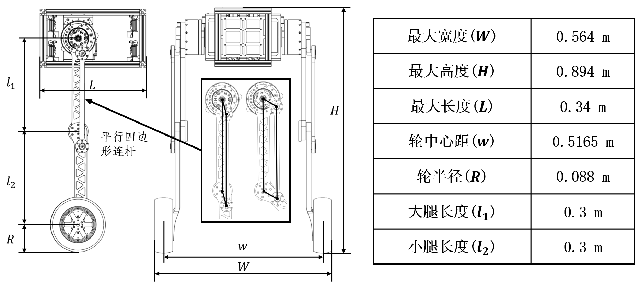
\includegraphics[width=0.4\linewidth]{figures/Sec2/dim.png}
%   \caption{
%   轮腿机器人的外形尺寸与主要杆件长度示意图。其中膝关节通过平行四边形连杆实现了远端驱动\cite{spong2006robot},减小了腿部的表征惯量(apparent inertia)。
%   }
%   \label{fig:sec2-dim}
%   \vspace{6pt}
% \end{figure}

% \begin{figure}
%   \centering
%   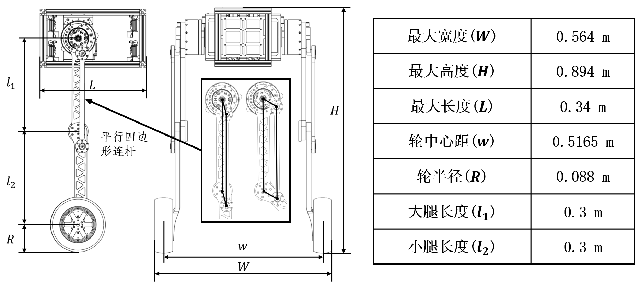
\includegraphics[width=0.4\linewidth]{figures/Sec2/dim.png}
%   \caption{
%   轮腿机器人的外形尺寸与主要杆件长度示意图。其中膝关节通过平行四边形连杆实现了远端驱动\cite{spong2006robot},减小了腿部的表征惯量(apparent inertia)。
%   }
%   \label{fig:sec2-dim}
%   \vspace{6pt}
% \end{figure}

如绪论中所述,本轮腿机器人的目标任务是在为人类设计的生活工作环境中辅助人类,例如物流、家务、看护等。考虑到某些任务并无法使用单独的轮腿来实现,如物流相关的任务需要机械臂以实现抓取移动、激光雷达和深度相机以实现物体识别和环境感知,因此本毕业设计的轮腿机器人主要是机器人底盘,负责具体实现基础的平衡与轨迹跟踪,后续相关功能如任务规划、避障或机械臂抓取等则可以在此平台基础上开发。在适合人类生活与工作的空间,最佳选择是与人类体型、体重相若的仿人机器人,但如绪论中所分析,其存在相当多的技术难点。因此轮腿机器人的设计目标是,身高与人类身高的一半相仿,尺寸与人类体型相近,且质量尽可能轻以提高机器人运动性能,增强续航。基于以上几点,轮腿机器人最终设计出来的尺寸如图\ref{fig:sec2-dim}所示。

\begin{figure}[h!]
  \centering
  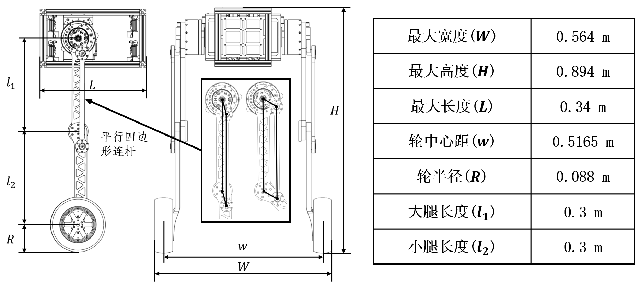
\includegraphics[width=0.9\linewidth]{figures/Sec2/dim.png}
  \caption{
  轮腿机器人的外形尺寸与主要杆件长度示意图。其中膝关节通过平行四边形连杆实现了远端驱动\cite{spong2006robot},减小了腿部的表征惯量(apparent inertia)。
  }
  \label{fig:sec2-dim}
   \vspace{6pt}
\end{figure}

考虑到机器人主要在室内场景工作,因此无需特别防水防尘设计。考虑到仅仅是原型机打样及,加工方式及预算较为宽裕,但需要频繁测试迭代,因此加工周期是重要考量因素,除了强度与精度要求高的结构件与配合使用CNC加工外,铝型材等预制件被广泛采用;此外,各种3D打印件也被使用在不同场景,如对韧性需求高的限位件使用尼龙3D打印,电机控制器、编码器的安装使用光固化或热熔沉积3D打印等等。

\begin{figure}
  \centering
  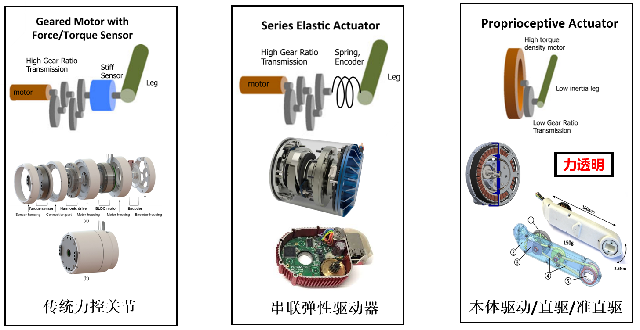
\includegraphics[width=0.7\linewidth]{figures/Sec2/force.png}
  \caption{
  轮腿机器人所使用的驱动器(电机),从左到右分别是胯部电机RMD-X8,定制膝盖电机和轮子电机AK-80-6.
  }
  \label{fig:sec2-force}
   \vspace{6pt}
\end{figure}

驱动系统是机器人运动的核心。考虑到液压驱动系统的难度高、体积大,不适合本毕业设计所期望的工况,因此本轮腿机器人计划采用电机驱动。而考虑到机器人后续的相关控制算法的应用,驱动电机需要具有力控功能。当前实现力控的方案一共有如图\ref{fig:sec2-force}所示的三种方案:传统力控关节,使用高减速比电机和力传感器实现,控制带宽高但无反驱能力,受到较大外力冲击易损坏传感器和减速器,应用于在KUKA iiwa\cite{bischoff2010kuka}和Kinova机械臂中;串联弹性驱动器(SEA)\cite{pratt1995series}使用双编码器测量弹性体形变间接测量力矩,具有柔性储能结构,耐受冲击,但高频力矩性能相应较弱;准直驱方案\cite{seok2012actuator}\cite{wensing2017proprioceptive}由于低减速比因此力透明,通过驱动器电流环直接进行力控,可以实现高频相应且抗冲击能力强,但输出扭矩密度不足。在三种方案间权衡,本毕业设计决定采用基于本体感知的准直驱电机作为力控方案,类似的方案被用在了麻省理工学院的Mini Cheetah机械狗\cite{katz2019mini}上,以及Agility Robotics推出的本体驱动双足机器人Cassie\cite{apgar2018fast-cassie}与Digit上。

\begin{figure}
  \centering
  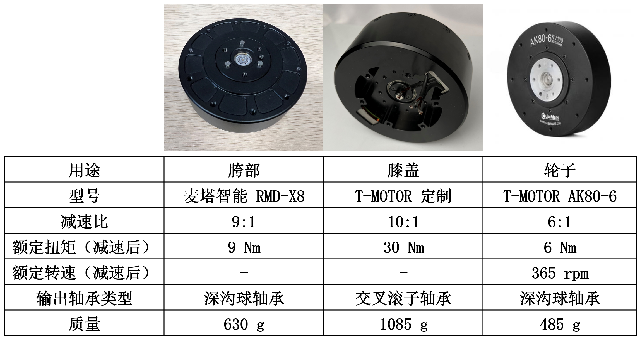
\includegraphics[width=0.9\linewidth]{figures/Sec2/motors.png}
  \caption{
  常见的三种力控机器人关节电机方案示意。
  }
  \label{fig:sec2-motors}
   \vspace{6pt}
\end{figure}

本轮腿机器人的创新点与电气部件中的驱动器(电动机)紧密相关,并且考虑到轮腿机器人膝关节需求扭矩大,市场上可供选择的驱动器种类少的限制条件,因此也需要根据实际驱动器选型调整轮腿的关键尺寸参数,如大腿和小腿的长度等等。如绪论中所述,本轮腿机器人的创新点之一在于使用准直驱实现所有驱动器的力矩控制。准直驱在绪论中已经有过叙述,在此不再赘述。考虑到机器人的膝关节扭矩最大,且准直驱要求电机减速比不能过高,因此最终膝关节选择了T-Motor定制电机(如图\ref{fig:sec2-motors}),具体参数在电气系统章节给出。该电机持续扭矩输出为30Nm(10:1减速之后),根据机器人预估质量进行静力学校核,并乘以安全系数之后,选定机器人的大腿及小腿长度,如上文图\ref{fig:sec2-dim}所示。


\subsection{轮腿机器人的结构设计}
如绪论所述,轮腿机器人的“腿”的部分的自由度有诸多选择,同时也有多种驱动器驱动形式,如Ascento机器人使用单个电机,但通过拓扑优化杆长,使用四杆机构实现上下运动;腾讯的Ollie机器人使用五杆并联机构,虽然活动范围小,但是单个电机所需扭矩并不是很大;而Handle机器人则拥有扭矩巨大的液压驱动器,因此可以使用与人或动物的腿最为相近的串联设计。在后续的子章节中,将会首先介绍自由度及驱动模块,然后是与相关的优化:远端驱动及连杆传动,最后介绍了轮腿机器人的活动范围(工作空间),以及限位的设计。

\subsubsection{自由度及驱动模块}
上一部分中,本毕设对比了几种电机布置形式与自由度的选择。考虑到轮腿机器人的用途,后续可能加装机械臂用来搬运物体,或动力尾以增强平衡能力与机动性,机器人的躯干部分(如图\ref{fig:sec2-dof-parts})的质心会经常改变。为了使机器人在质心改变之后仍能再视觉上保持躯干的竖直状态,这一点对于激光雷达、深度相机进行环境感知提供了便利和持续一致的视野,我们选择使用2自由度的腿部设计。否则如果采用单自由度仅能变高度的设计,则需要在改变负载时精心调整负载位置,或使机器人整体在一个倾斜的角度平衡,前者是运送货物时难以做到的,而后者则是感知时不希望看到的。
综上所述,本毕设提出的机器人将会有每条腿2个自由度,轮子1个自由度,总共6个自由度的设计,如图\ref{fig:sec2-dof-parts}所示。在这里需要说明的是,使用并联的5杆机构同样可以实现上述需求,并且并联机构能够使电机合力更大,但是考虑到结构的简单性,并考虑到已有性能较强的电机,本毕设使用的是串联构型。

\begin{figure}
  \centering
  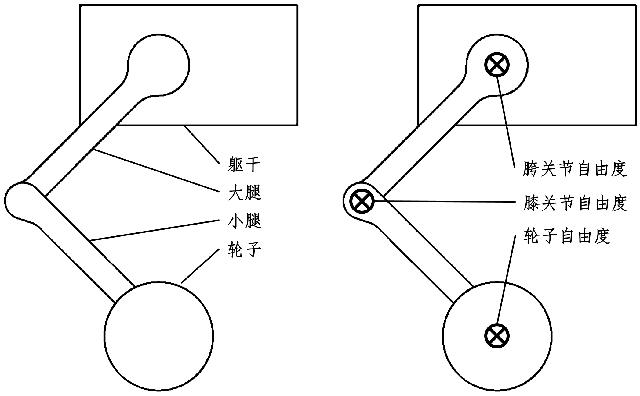
\includegraphics[width=0.75\linewidth]{figures/Sec2/dof-parts.png}
  \caption{
  左图:轮腿机器人可以分成躯干、大腿、小腿、轮子几个部分,之后也会用这些名称来代指。右图:轮腿机器人的自由度分布,分别是轮子、膝盖、胯部。
  }
  \label{fig:sec2-dof-parts}
   \vspace{7pt}
\end{figure}

在本章的引言中,膝关节的驱动模块已经被粗略介绍过了,与其他机器人驱动器的具体技术细节一起,将在电气系统章节给出。这里的选型依据是综合考量输出扭矩、最大转速、减速器齿隙、输出配合然后决定的。值得注意的是,电磁电动机的扭矩与体积有如下固定的上限关系如公式\ref{eq:motor-tau-vol}\cite{hughes2006electric}所示,其中$D^2L$与体积成正比。
\begin{equation}
    T = (\bar{A}\bar{B})\times (\pi DL) \times D / 2 = \frac{\pi}{2} (\bar{A}\bar{B}) D^2 L
    \label{eq:motor-tau-vol}
\end{equation}
而减速器的加入可以增加电机的输出扭矩,但也会减少力的透明传输特性与反驱能力,因此减速比的选择也是重要的考量因素。
膝关节驱动器具有特殊性,这里不再赘述。轮子电机选用T-Motor的AK80-6(如图\ref{fig:sec2-motors}),考虑到轮子并无需提供很大扭矩,但需要有较快的转速,因此选用尺寸、功率合适而减速比为6:1的该型号电机。由于胯部电机安装在躯干上,同时负责驱动躯干的旋转,选择的侧重点则是自重和扭矩,因此选择了尺寸、功率合适的9:1减速比的麦塔智能的RMD-X8电机(如图\ref{fig:sec2-motors})。这两个电机的输出配合、安装方式、常见工况将在下一子章节中详细展开。膝盖电机在上文已经介绍过,也将在电气章节详细展开。

\subsubsection{远端驱动及连杆传动}
% 机器人整体结构设计图及平行连杆结构
在确定了自由度与驱动器之后,驱动器的位置布置与传动方式的选择将在本节讨论。考虑到本轮腿属于验证原型机性质,驱动方式尽量从简,且轮子和胯部电机本身就是带有减速器的QDD电机,因此它们通过合适的关节和连接件直接驱动对应的轮毂和大腿杆件。而考虑到膝关节电机质量较大,为减少系统建模与控制难度,减少表征惯量,考虑了运动范围和扭矩,将电机布置在远端(躯干位置,与胯部电机同心),采用平行四边形连杆机构传动,具体如图\ref{fig:sec2-dim}所示。值得注意的是,考虑到运动范围与轮腿机器人常见位姿,以及小腿的加工复杂度,选择了当前平行四边形的短杆长度。这样在增加限位之后(在下一节会介绍限位),连杆不会达到奇异位置,而膝关节驱动器便可等效安装在膝关节位置而不是远端。在后文的建模和控制章节中,运动学也可以进行等效,动力学也可以进行简化。

\subsubsection{活动范围及限位设计}
对于串联结构的腿式机器人,膝盖弯曲方向也是应当考虑的。人类的膝盖是向前弯曲的,而马、鸵鸟等动物的趾骨也是腿的一部分,因此可以观察到向后弯曲的腿。笔者认为,对于无需通过步态实现移动的轮腿机器人,由于大腿与小腿的长度相等,因此膝盖的方向选择更多需要考虑实际工作情况。考虑到后续可能在轮腿机器人上安装机械臂,例如需要靠近桌子使用机械臂夹取桌上物品(如图\ref{fig:sec2-table}所示),因此选择膝盖后弯的形式。和在绪论中介绍的一样,Handle机器人(图\ref{fig:sec1-Handle})和Ascento机器人(图\ref{fig:sec1-Ascento})也都采用膝盖后弯的形式。

\begin{figure}[h!]
  \centering
  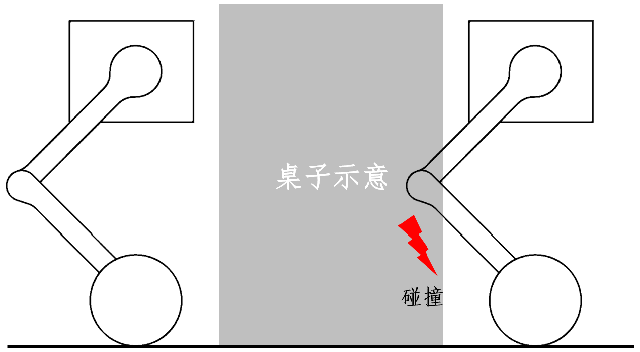
\includegraphics[width=0.75\linewidth]{figures/Sec2/table.png}
  \caption{
  如图所示,如果机器人需要靠近桌子使用机械臂夹取桌子上的物体,则膝盖向后完全的形式比膝盖向前弯曲的形式有更大概率免于碰撞。
  }
  \label{fig:sec2-table}
   \vspace{5pt}
\end{figure}

上一章节有关连杆设计的部分,对于膝盖前弯和后弯而言都可以使用相同的参数,区别在于连杆的布置位置朝前或朝后。在确定了膝盖弯曲的方向之后,也便可以定义机器人的前后、左右、上下,也就是矢状面、冠状面、横断面,如图\ref{fig:sec2-3lim}所示。因此膝盖限位可以直接设计在连杆上,使用尼龙3D打印,以兼顾刚性、韧性和弹性。在后续实验章节的系统集成子章节中,将会介绍基于状态机的电流及位置限制器,以确保电机不会撞到限位或以较大扭矩挤压限位,因此这里的机械限位除了作为最后一道安全限位措施外,主要实现了机器人下电状态下支撑机器人和绝对位置编码器校准的作用。在轮腿机器人的膝盖电机在静能状态下,电机完全不输出扭矩,限位件支撑机器人到最低高度,轮子和膝盖保护件与地面接触,支撑机器人,膝盖保护件采用硬度较高且较光滑的尼龙3D打印件制作,实现了双轮差速车的效果。

\begin{figure}
  \centering
  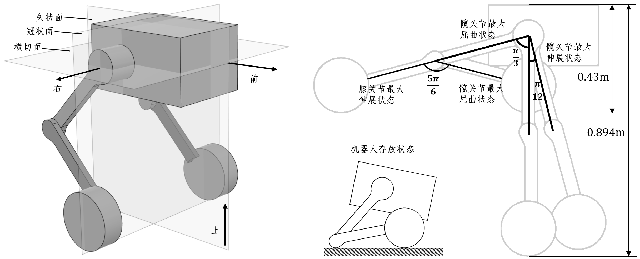
\includegraphics[width=1.0\linewidth]{figures/Sec2/3lim.png}
  \caption{
  左图:轮腿机器人的矢状面、冠状面和横切面,以及相应的前、右、上方向。右图:机器人的膝关节和髋关节的限位大小及机器人平衡时的最大最小高度,左下则是当机器人关闭电源时,凭借关节限位与膝盖支撑件保持摆放状态。
  }
  \label{fig:sec2-3lim}
   \vspace{7pt}
\end{figure}


胯部的限位件的设计考虑了在整个机器人可变高度的范围内,需要通过胯部电机和膝盖电机配合以确保机器人躯干竖直向上。因此胯部限位件在某一方向限制胯部电机的运动幅度与膝盖电机的运动幅度相关,而在另一方向则选择了一个较小的值,以实现如前文所述的在一定范围内调整重心的需求。
膝盖限位件需要限制膝盖电机的运动范围在180°以内,以防止连杆机构奇异,但实际上接近竖直的状态连杆会对限位件产生巨大的压力而导致形变,使连杆系统处于奇异状态,因此在本原型机中,将膝盖电机的运动范围限制在以完全折叠为0°的30°到180°范围内。根据前文所述,胯部限位件将胯部电机的活动范围限制在以竖直位置为0°的-75°到15°的范围内,如图\ref{fig:sec2-3lim}所示。

\subsection{轮腿机器人的机械设计}
在本子章节中,将会介绍轮腿机器人的具体设计,包括CNC结构件的设计、减重与强度校核,不同3D打印件的用途与设计,然后介绍了关节和连接件的设计与配合。这些机械设计的图纸与3D打印零件的示意图会附在附录中。

\subsubsection{结构件设计及强度校核}
在前面的子章节中,轮腿机器人的大腿和小腿长度都已经确定了,同时考虑到远端驱动的连杆设计,小腿的宽度也已经确定。为了追求视觉的一致性,大腿的宽度与小腿选择一致。在此基础上,厚度与镂空方式将根据经验选择,然后再通过有限元仿真进行强度校核。本轮腿设计使用的CAD软件使Autodesk公司的Fusion 360,内置静力学仿真,根据机器人的典型重量和重力、宽度产生的扭矩对小腿和大腿的目前设计进行了强度校核,如图\ref{fig:sec2-simu}所示。

\begin{figure}
  \centering
  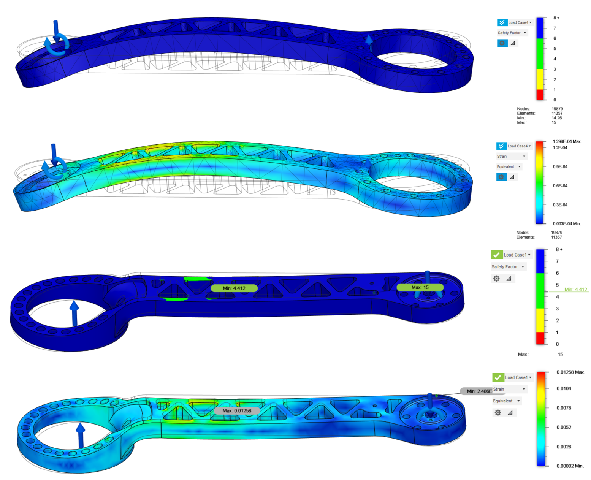
\includegraphics[width=0.85\linewidth]{figures/Sec2/simu.png}
  \caption{
  上2张图:大腿杆件在有限元仿真中的静力学负载工况下的安全系数和应变。值得注意的是图中所展示的形变是夸张的展示形变的趋势而远非实际情况。下2张图:小腿杆件在有限元仿真中的静力学负载工况下的安全系数和应变。
  }
  \label{fig:sec2-simu}
   \vspace{5pt}
\end{figure}

值得注意的是,上述的扭矩和重力在设计关节和连接件如轴承的选用时,也将同样纳入考量范围。

\begin{figure}[h!]
  \centering
  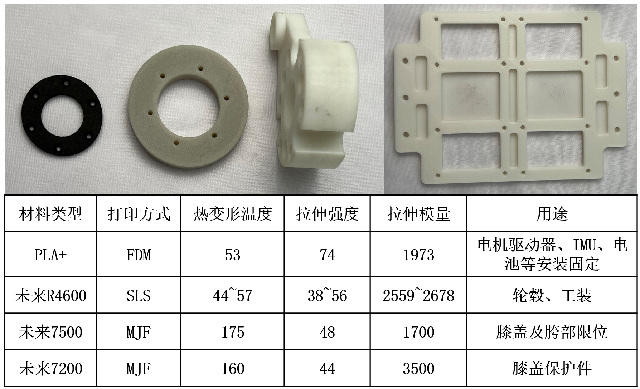
\includegraphics[width=0.85\linewidth]{figures/Sec2/3dp.png}
  \caption{
  上图从左到右依次是未来7500,未来7200,未来R4600及PLA+,下图则是这些3D打印材料的机械性能及使用用途。
  }
  \label{fig:sec2-3dp}
   \vspace{6pt}
\end{figure}

所有3D打印件的材料、用于、机械性能如图\ref{fig:sec2-3dp}所示,上文已经提到过膝盖支撑3D打印件,这里不再赘述。膝盖限位件的设计与远端驱动的连杆在到达限位的位置进行平面的配合,如图\ref{fig:sec2-2lim}所示,而胯部限位件则采用两个圆弧面与胯部电机的输出盘配合以起到限位的效果,如图\ref{fig:sec2-2lim}所示。在下一节中,将会介绍包括电机输出在内的连接件,而本轮腿机器人的轮胎和胎皮都采用RC现成产品,而轮毂则由3D打印制成。关于轮毂的设计的细节将在下一节中详细展开。电机编码器、电机驱动器、IMU、电池等机电部件也广泛使用3D打印配件固定,和躯干上的铝型材保护框架,都将在下一子章节介绍。

\begin{figure}
  \centering
  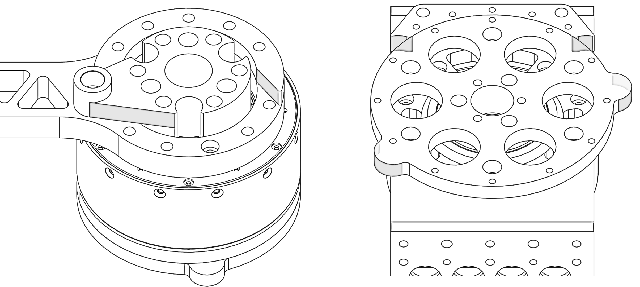
\includegraphics[width=0.85\linewidth]{figures/Sec2/2lim.png}
  \caption{
  膝盖和胯部的限位设计。
  }
  \label{fig:sec2-2lim}
   \vspace{6pt}
\end{figure}

\subsubsection{关节设计与连接件选择}
在本节中,主要包括轮腿的关节,及关节的连接件,如膝关节使用的交叉滚子轴承,各电机输出盘的配合,连杆的轴承选择与配合等等。
如上文所述,轮子电机选用的时T-Motor的AK80-6,其具有内置的行星减速箱,输出轴为一个深沟球轴承。为了优化电机安装厚度通过设计轮毂使得轮胎中心过电机输出的深沟球轴承,从而使该轴承主要承受因重力而产生的径向力,在轮腿机器人转弯时需要承受较小的轴向力。而该设计使得轴承无需承受转矩,从而无需额外轴承及配合,如图\ref{fig:sec2-mech}所示,使得轮子设计更为紧凑。考虑到轮毂的加工难度和快速打样的需求,采用光固化的3D打印加工,但是其表面硬度不足,与直径较小销进行配合后,当电机输出较大扭矩时,容易使轮毂形变从而导致背隙。因此本设计采用多颗直径较大的塞达螺丝与轮毂配合的形式。

\begin{figure}
  \centering
  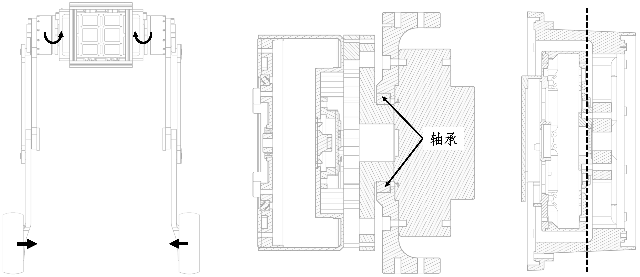
\includegraphics[width=0.85\linewidth]{figures/Sec2/mech.png}
  \caption{
  左图:当轮胎受到同向的力时,将在胯部产生巨大扭矩。中图:胯部的双轴承设计,分别是图中所示轴承与电机输出轴轴承。右图:通过设计3D打印的轮毂,使得轮子中心过轮子电机的轴承,从而免去双轴承设计,且使布局更为紧凑。
  }
  \label{fig:sec2-mech}
   \vspace{6pt}
\end{figure}

膝关节采用冠林的XRU1008交叉滚子轴承,该类型的轴承可以提供较大的所有方向的力和矩的支撑。为方便安装选用预置螺纹孔和通孔的版本,且该轴承外壁与大腿配合以弥补通孔同心度不足的问题,而一个额外的钢件与内径配合,并通过螺丝固连置小腿,增强强度。
连杆轴承选用6001深沟球轴承,膝盖电机输出盘通过花键与平行四边形连杆配合,大腿与膝盖通过若干颗螺丝连接,其中两颗为塞打螺丝,以实现同心度定位。由于定制电机尾部安装孔没有定位特征,因此通过一个3D打印的高精度工装安装到一个转接盘上,从而与胯部电机的输出转接件通过16颗螺丝进行定位。而胯部电机使用输出盘自带3个定位销,因此可以使用此与之定位。但值得注意的是,膝盖电机仅需输出纯扭矩,而胯部电机则在输出扭矩的同时需要轴承提供用于对抗重力弯矩的扭矩,另外当两个轮子受到同时向内或向外的力时,胯部电机的轴承需要提供巨大的扭矩,如图\ref{fig:sec2-mech}所示,因此在胯部输出转接件上额外安装了一个6808轴承以和电机输出轴承实现双轴承的效果,提高了抗弯能力。
上一节提到的限位件在绝对位置编码器校准时有重要作用,因此也需要考虑其配合关系。本设计中,膝关节和髋关节的限位都使用塞达螺丝定位。而髋关节电机的同心通过电机自带的凸台特征确保。考虑到躯干的上下板将会安装感知元器件或机械臂,对定位也有一定要求,因此上下板与胯部电机安装座之间的定位采用大头销,便于安装。

\subsection{轮腿机器人的机电设计}
在本章节中,将会介绍与电气相关的零部件的布置与安装。关于电气零部件的详细信息将会在第二章展开。

所有电机均需要安装磁编码器,其中膝盖和胯部电机自带磁铁,且其使用的绝对位置编码器自带安装盘,可以直接安装;而轮子电机需要首先拆除T-Motor原装驱动板,使用3D打印件安装此贴和相对位置编码器。另外需要安装的电气相关的配件是电机驱动器、IMU及通讯单片机PCB、遥控急停、电池及SpeedGoat控制器。

为了安装这些设备,并在机器人可能摔倒的情况下保护,同时考虑快速打样原型机,使用铝型材制作框架,然后使用3D打印件安装电机驱动器与SpeedGoat控制器至框架上。而IMU的安装位置则需要考虑机器人的运动与IMU各轴读数的解耦,例如当机器人围绕中心自转时,IMU应当仅有偏航角发生改变。电池安装在电池架上,而电池架也通过3D打印件安装在机器人躯干上。

\subsection{本章小结}

本章中,首先介绍了机器人的工作环境,也就是相关的机械设计约束,然后介绍了电机系统相比于液压系统的优点及选择原因,在此基础上对比了常见的三种电机实现力控方案,及选择QDD作为力控实现的原因。通过对工况的分析确定了机器人整体尺寸、自由度和构型布置,并通过对电机的粗选型细化了上述机器人参数。据此可以开始细致设计机器人,包括结构件的强度、配合、加工工艺,机电系统整体设计等等。